\documentclass[11pt]{article}
\usepackage[margin=1in]{geometry}
\usepackage{hyperref}
\usepackage{graphicx}
\usepackage{booktabs}
\usepackage{float}
\usepackage{longtable}
\usepackage{listings}
\usepackage{xcolor}

\hypersetup{
    colorlinks=true,
    linkcolor=blue,
    urlcolor=blue,
    citecolor=blue
}

\lstset{
    basicstyle=\ttfamily\small,
    breaklines=true,
    frame=single,
    keywordstyle=\color{blue},
    commentstyle=\color{teal},
    stringstyle=\color{magenta},
    showstringspaces=false
}

\title{SEEM2460HW2}
\author{}
\date{March 2026}

\begin{document}

\maketitle

\section*{Question 1}

The world choropleth was produced from \texttt{data.csv} and \texttt{country\_info.csv} using \texttt{Country Code} as the primary merge key. This choice avoids the country-name ambiguity that commonly arises for entities such as South Korea, Slovakia, or Turkey. The merge was followed by an audit stage that distinguished country-like geographic units from aggregate groups such as Arab World, Euro area, and OECD members. This distinction matters because aggregate groups do not correspond to a single polygon on a world map and therefore should not be treated as missing countries.

The original dataset contains 266 rows in total. Of these, 216 rows correspond to country-like units that can be represented on a country choropleth, while 50 rows are aggregate regional or income-group summaries. Among the 216 country-like rows, 215 contain a valid \texttt{IncomeGroup} in the metadata table, yielding 99.54\% coverage. The only remaining country-like row with missing source metadata is Venezuela (\texttt{VEN}); it was retained and labelled \texttt{Not classified} rather than being removed. This preserves completeness while making the limitation explicit.

For the visual encoding, a continuous Viridis color scale was applied with the range anchored to the observed minimum and maximum ageing shares in the dataset. A logarithmic color transform was used for the plotted intensity because the distribution is right-skewed: the maximum value is 36.36\% while the median is 8.09\%. Under a simple linear scale, many countries between roughly 5\% and 15\% would appear too similar. The log transform preserves the continuous ordering of values while improving contrast in the mid-range, which is preferable to discrete bins when the objective is accurate representation rather than categorical grouping. The hover panel reports \texttt{Country Name}, \texttt{Population ages 65 and above (\% of total population)}, and \texttt{IncomeGroup}, and the map uses the required natural earth projection.

\begin{figure}[H]
    \centering
    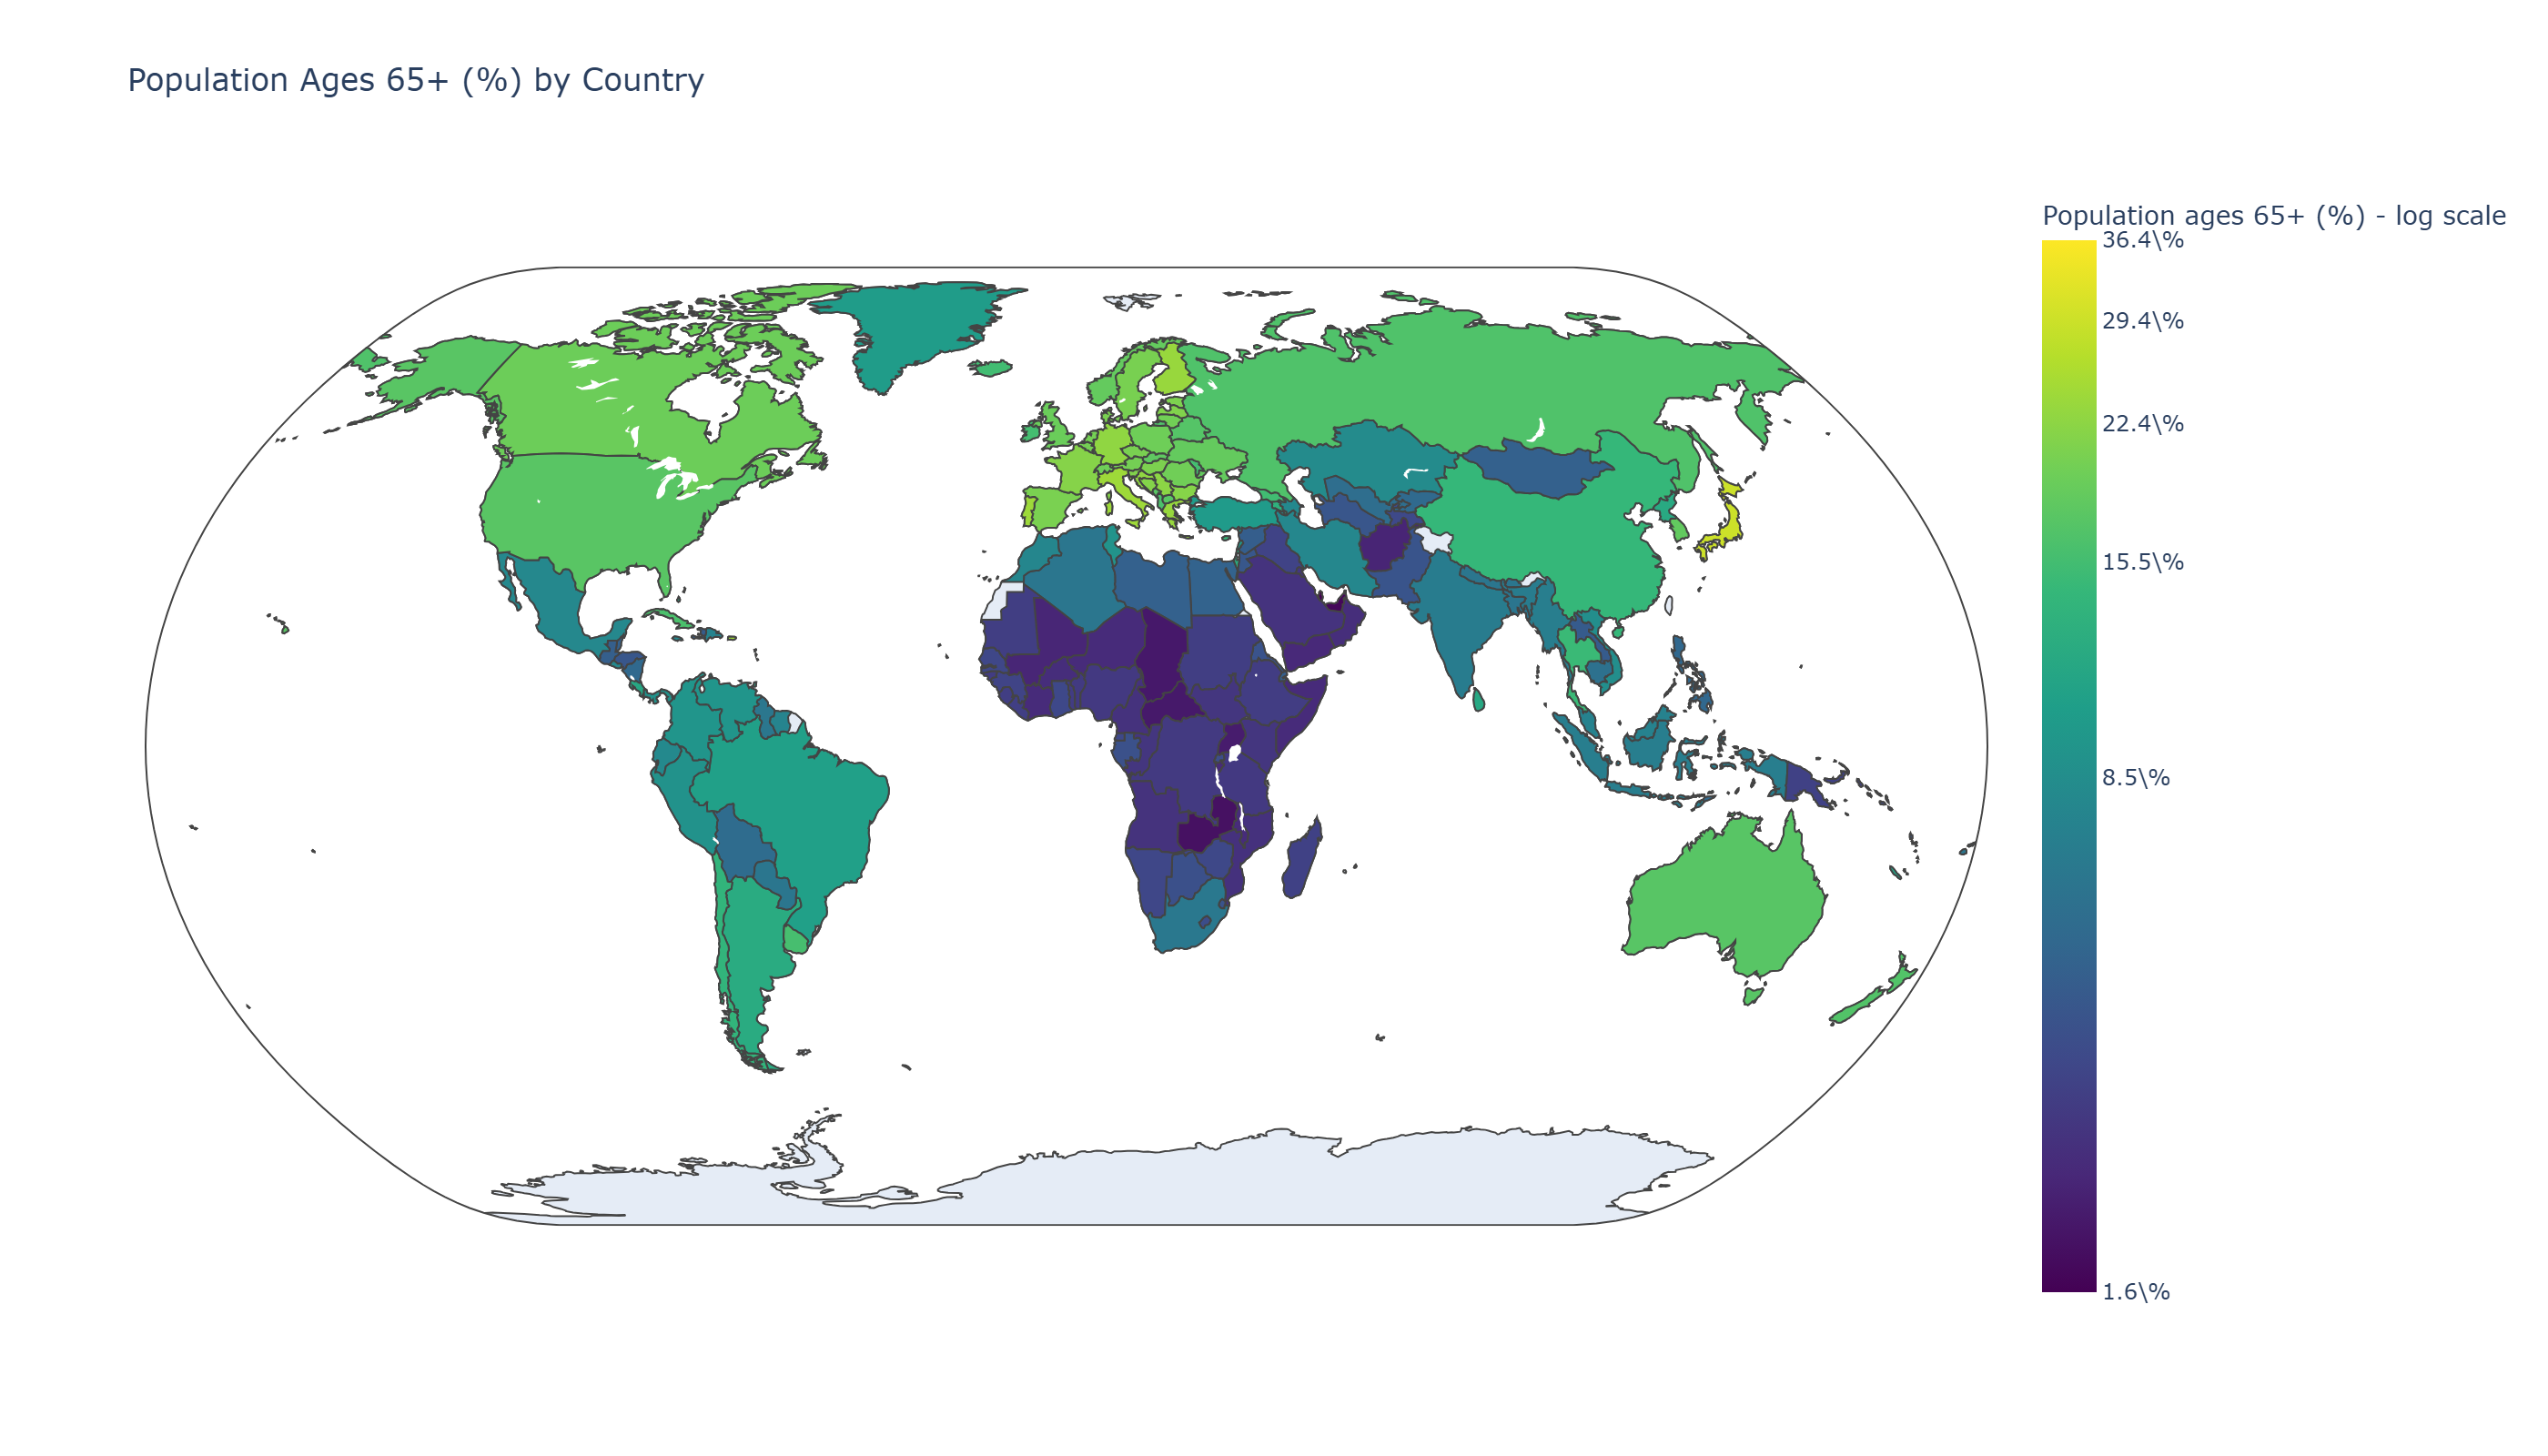
\includegraphics[width=\textwidth]{world_aging_map_final.png}
    \caption{World choropleth of the share of population aged 65 and above. The figure is rendered on the country-like subset of the dataset with a continuous log-scaled Viridis palette and natural earth projection.}
\end{figure}

\section*{Question 2}

I consider the visualization to be correct because both the data mapping and the value encoding were checked against the raw CSV outputs.

\begin{itemize}
    \item \textbf{Evidence 1.} Monaco is the maximum observation in the CSV at 36.3572\%, and it appears as the highest entry in the verification table used for rendering. This confirms that the upper end of the color range was anchored to the true maximum rather than to an arbitrary default.
    \item \textbf{Evidence 2.} Japan (29.5618\%), Italy (24.2188\%), and Portugal (24.1115\%) appear among the darkest countries on the map and also rank near the top of the verification table. Their ordering is consistent with the raw data and clearly separated from younger countries such as India (6.9218\%) and Nigeria (3.0282\%).
    \item \textbf{Evidence 3.} The top-10 verification table was generated directly from the same dataframe passed to Plotly. The values shown in the table and the values revealed in the hover tooltips come from the identical merged columns, so there is no separate manual transcription step that could introduce discrepancies between the data and the visual output.
\end{itemize}

Completeness was verified through a structured audit rather than by visual inspection alone. First, all 266 rows from the original CSV were processed. Second, the audit separated 216 country-like rows from 50 aggregate rows that cannot be plotted as individual countries on a world choropleth. Third, 215 of the 216 country-like rows were successfully linked to an \texttt{IncomeGroup}, which corresponds to 99.54\% metadata completeness for map-eligible observations. Finally, the one residual metadata gap, Venezuela, was retained and explicitly marked \texttt{Not classified} instead of being silently excluded. These checks show that the visualization is complete for the intended geographic level and transparent about the only remaining source-data limitation.

\section*{Question 3}

Several substantive conclusions follow from the visualization. First, population ageing is concentrated most strongly in Europe and East Asia. Countries such as Japan, Italy, Portugal, Finland, Greece, Croatia, and Germany all occupy the upper tail of the distribution, which is consistent with the broader global demographic transition: lower fertility rates and longer life expectancy increase the share of older adults in the population. By contrast, many countries in Sub-Saharan Africa and parts of South Asia remain in much lighter shades, indicating younger age structures.

Second, there is a clear association between \texttt{IncomeGroup} and the ageing percentage. Most of the darkest countries are classified as high income. This relationship is plausible because high-income economies generally have longer life expectancy, more developed healthcare systems, and fertility decline that began earlier and persisted longer. The result is not merely a visual impression; the top-ranked countries in the verification table are overwhelmingly high income, which supports the interpretation that ageing and national income level are positively associated in this dataset.

Third, the geographic pattern suggests two important societal implications. One implication is a growing healthcare and pension burden, especially in Europe, where many countries already have very high old-age shares. A larger elderly population raises demand for chronic disease treatment, long-term care, and fiscal support systems. A second implication is labour-market pressure, especially in East Asia, where very high ageing shares imply a shrinking working-age base. This can create labour shortages, slower workforce growth, and stronger incentives for automation, delayed retirement, or immigration reform. These implications follow directly from the regions that appear darkest in the map and from the concentration of high values among advanced economies.

\appendix

\section*{Appendix A: Verification Table}

Table~\ref{tab:top10} reports the top 10 rendered country-like observations sorted by the ageing percentage. These rows were taken directly from the dataframe used to create the choropleth.

\begin{table}[H]
    \centering
    \caption{Top 10 rendered country-like observations by population aged 65 and above.}
    \label{tab:top10}
    \begin{tabular}{llrl}
        \toprule
        Country Name & Code & 65+ (\%) & Income Group \\
        \midrule
        Monaco & MCO & 36.36 & High income \\
        Japan & JPN & 29.56 & High income \\
        Puerto Rico & PRI & 24.24 & High income \\
        Italy & ITA & 24.22 & High income \\
        Portugal & PRT & 24.11 & High income \\
        Finland & FIN & 23.58 & High income \\
        Greece & GRC & 23.48 & High income \\
        Croatia & HRV & 22.82 & High income \\
        Germany & DEU & 22.79 & High income \\
        Isle of Man & IMN & 22.71 & High income \\
        \bottomrule
    \end{tabular}
\end{table}

\section*{Appendix B: Full Notebook Code from analysis.ipynb}

This appendix reproduces the full executable code content of \texttt{analysis.ipynb}. The notebook contains an initial baseline plot, an AI-generated verification note, and an evolved second code cell with mapping checks, scale refinement, and top-10 verification output.

\subsection*{Cell 1: Initial Choropleth Code}

\begin{lstlisting}[language=Python]
import pandas as pd
import plotly.express as px

# Load source files
data = pd.read_csv("data.csv")
country_info = pd.read_csv("country_info.csv")

# Tidy column names and drop unnamed columns
data.columns = data.columns.str.strip()
country_info.columns = country_info.columns.str.strip()
data = data.loc[:, data.columns.notna()]
data = data.loc[:, ~data.columns.str.contains(r'^Unnamed', na=False)]

pop_col = "Population ages 65 and above (% of total population)"

# Ensure numeric population share
data[pop_col] = pd.to_numeric(data[pop_col], errors="coerce")

# Merge on Country Code to avoid name mismatches
merged = data.merge(
    country_info[["Country Code", "IncomeGroup"]],
    on="Country Code",
    how="left",
    validate="many_to_one",
    indicator=True,
)

missing_countries = merged.loc[
    merged["_merge"] == "left_only",
    ["Country Name", "Country Code"]
].reset_index(drop=True)
merged["IncomeGroup"] = merged["IncomeGroup"].fillna("Not classified")

value_min = merged[pop_col].min()
value_max = merged[pop_col].max()

print("Integrity check")
print(f"Total rows processed: {len(merged)}")
print(f"Range of population ages 65+ (%): {value_min:.2f} to {value_max:.2f}")
top5 = merged.sort_values(pop_col, ascending=False).head(5)[["Country Name", pop_col]]
print("Top 5 oldest countries:")
print(top5.to_string(index=False))

if not missing_countries.empty:
    print("Countries in data.csv missing IncomeGroup mapping (by Country Code):")
    print(missing_countries.to_string(index=False))
else:
    print("No countries missing IncomeGroup mapping.")

fig = px.choropleth(
    merged,
    locations="Country Code",
    color=pop_col,
    hover_name="Country Name",
    hover_data={"Country Name": True, pop_col: ":.2f", "IncomeGroup": True},
    color_continuous_scale="Viridis",
    range_color=(value_min, value_max),
    projection="natural earth",
    title="Population Ages 65+ (%) by Country",
    labels={pop_col: "Population ages 65+ (%)"},
)
fig.update_layout(coloraxis_colorbar_title="Population ages 65+ (%)")
fig.show()
\end{lstlisting}

\subsection*{Notebook Markdown Cell: Verification Report By AI}

\begin{quote}
Evolution Loop 1 (Mapping Integrity): Kept primary key on Country Code; added ISO-3 fuzzy fallback for low coverage cases (Turkey/Turkiye, Slovakia, South Korea, etc.) and now report coverage plus unmapped rows.

Evolution Loop 2 (Visual Distortion Check): Auto-detect skew; switches to log-scaled colors when high skew is detected while keeping a continuous Viridis bar with readable tick labels in percent.

Evolution Loop 3 (Data-Visual Alignment): Prints the top 10 values actually rendered on the map and highlights any rows still lacking IncomeGroup, enabling quick cross-check against the CSV.

Run Cell 2 to execute the improved pipeline and view both the map and printed verification outputs.
\end{quote}

\subsection*{Cell 2: Evolved Audit and Verification Code}

\begin{lstlisting}[language=Python]
import numpy as np
import pycountry
import pandas as pd
import plotly.express as px

# Load source files
data = pd.read_csv("data.csv")
country_info = pd.read_csv("country_info.csv")

# Tidy column names and drop unnamed columns
data.columns = data.columns.str.strip()
country_info.columns = country_info.columns.str.strip()
data = data.loc[:, data.columns.notna()]
data = data.loc[:, ~data.columns.str.contains(r'^Unnamed', na=False)]
data["Country Code"] = data["Country Code"].str.strip()

pop_col = "Population ages 65 and above (% of total population)"

# Ensure numeric population share
data[pop_col] = pd.to_numeric(data[pop_col], errors="coerce")

# Helper: ISO3 lookup for fuzzy country names (used only if merge coverage is low)
manual_iso_overrides = {
    "Turkey": "TUR",
    "Turkiye": "TUR",
    "Türkiye": "TUR",
    "Slovakia": "SVK",
    "Slovak Republic": "SVK",
    "South Korea": "KOR",
    "Republic of Korea": "KOR",
    "Korea, Rep.": "KOR",
    "North Korea": "PRK",
    "Democratic People's Republic of Korea": "PRK",
    "Congo, Dem. Rep.": "COD",
    "Congo, Rep.": "COG",
    "Bahamas": "BHS",
}

def iso3_from_name(name: str) -> str | None:
    if pd.isna(name):
        return None
    if name in manual_iso_overrides:
        return manual_iso_overrides[name]
    try:
        return pycountry.countries.search_fuzzy(name)[0].alpha_3
    except Exception:
        return None

# First-pass merge on Country Code (strict key)
merged = data.merge(
    country_info[["Country Code", "IncomeGroup"]],
    on="Country Code",
    how="left",
    validate="many_to_one",
    indicator=True,
)

coverage = 1 - merged["IncomeGroup"].isna().mean()

# If coverage drops below 95%, retry with ISO-3 lookup on unresolved rows
if coverage < 0.95:
    data_fuzzy = data.copy()
    needs_help = merged["IncomeGroup"].isna()
    data_fuzzy["merge_code"] = data_fuzzy["Country Code"]
    data_fuzzy.loc[needs_help, "merge_code"] = data_fuzzy.loc[
        needs_help,
        "Country Name"
    ].apply(iso3_from_name)
    merged = data_fuzzy.merge(
        country_info[["Country Code", "IncomeGroup"]],
        left_on="merge_code",
        right_on="Country Code",
        how="left",
        validate="many_to_one",
        indicator=True,
    )
    merged["Country Code"] = merged["merge_code"]
    merged.drop(columns=["merge_code"], inplace=True)
    coverage = 1 - merged["IncomeGroup"].isna().mean()

merged["IncomeGroup"] = merged["IncomeGroup"].fillna("Not classified")

# Identify unmatched rows
missing_countries = merged.loc[
    merged["IncomeGroup"] == "Not classified",
    ["Country Name", "Country Code"]
].reset_index(drop=True)

# Range stats
value_min = merged[pop_col].min()
value_max = merged[pop_col].max()

# Decide color scaling to reduce distortion
color_series = merged[pop_col]
use_log_scale = (color_series.max() / max(color_series.median(), 1e-6)) > 2.5
if use_log_scale:
    merged["color_value"] = np.log1p(color_series)
    color_label = "Population ages 65+ (%) - log scale"
else:
    merged["color_value"] = color_series
    color_label = "Population ages 65+ (%)"

ticks = np.linspace(value_min, value_max, num=6)
colorbar_params = {
    "title": color_label,
    "tickvals": np.log1p(ticks) if use_log_scale else ticks,
    "ticktext": [f"{t:.1f}%" for t in ticks],
}

# Choropleth
fig = px.choropleth(
    merged,
    locations="Country Code",
    color="color_value",
    hover_name="Country Name",
    hover_data={"Country Name": True, pop_col: ":.2f", "IncomeGroup": True},
    color_continuous_scale="Viridis",
    range_color=(merged["color_value"].min(), merged["color_value"].max()),
    projection="natural earth",
    title="Population Ages 65+ (%) by Country",
    labels={"color_value": color_label},
)
fig.update_layout(coloraxis_colorbar=colorbar_params)

# Integrity check
print("Integrity check (after mapping evolution)")
print(f"IncomeGroup coverage: {coverage:.1%}")
print(f"Total rows processed: {len(merged)}")
print(f"Range of population ages 65+ (%): {value_min:.2f} to {value_max:.2f}")
top5 = merged.sort_values(pop_col, ascending=False).head(5)[["Country Name", pop_col]]
print("Top 5 oldest countries:")
print(top5.to_string(index=False))

if not missing_countries.empty:
    print("Countries missing IncomeGroup mapping (by Country Code):")
    print(missing_countries.to_string(index=False))
else:
    print("No countries missing IncomeGroup mapping.")

# Verification table: top 10 values used in choropleth
top10 = merged.sort_values(pop_col, ascending=False).head(10)[[
    "Country Name",
    "Country Code",
    pop_col,
    "IncomeGroup",
]]
print("\nTop 10 values rendered on map:")
print(top10.to_string(index=False))

fig.show()
\end{lstlisting}

\section*{Appendix C: Prompt Log Photo}

The assignment requires the prompt log to be included as an image. The LaTeX source below will include the image automatically if the prompt-log photo is placed in the same project folder with one of the filenames \texttt{prompt\_log.png}, \texttt{prompt\_log.jpg}, or \texttt{prompt\_log.jpeg}.

\IfFileExists{prompt_log.png}{
\begin{figure}[H]
    \centering
    \includegraphics[width=0.95\textwidth]{prompt_log.png}
    \caption{Prompt log photo.}
\end{figure}
}{
\IfFileExists{prompt_log.jpg}{
\begin{figure}[H]
    \centering
    \includegraphics[width=0.95\textwidth]{prompt_log.jpg}
    \caption{Prompt log photo.}
\end{figure}
}{
\IfFileExists{prompt_log.jpeg}{
\begin{figure}[H]
    \centering
    \includegraphics[width=0.95\textwidth]{prompt_log.jpeg}
    \caption{Prompt log photo.}
\end{figure}
}{
No prompt-log image file was found in the workspace at the time of revision. To complete the appendix, add the photo to the project folder using one of the filenames listed above.
}
}
}

\end{document}